\chapter{Post installation}
\label{chapter:post_install}

\section{Update RegaDB with the latest auxilary data}
Navigate your browser to \textit{http://localhost:8080/regadb/RegaDB}, and login to the system.
\\
\vspace{0.5cm}~ \\ \centerline{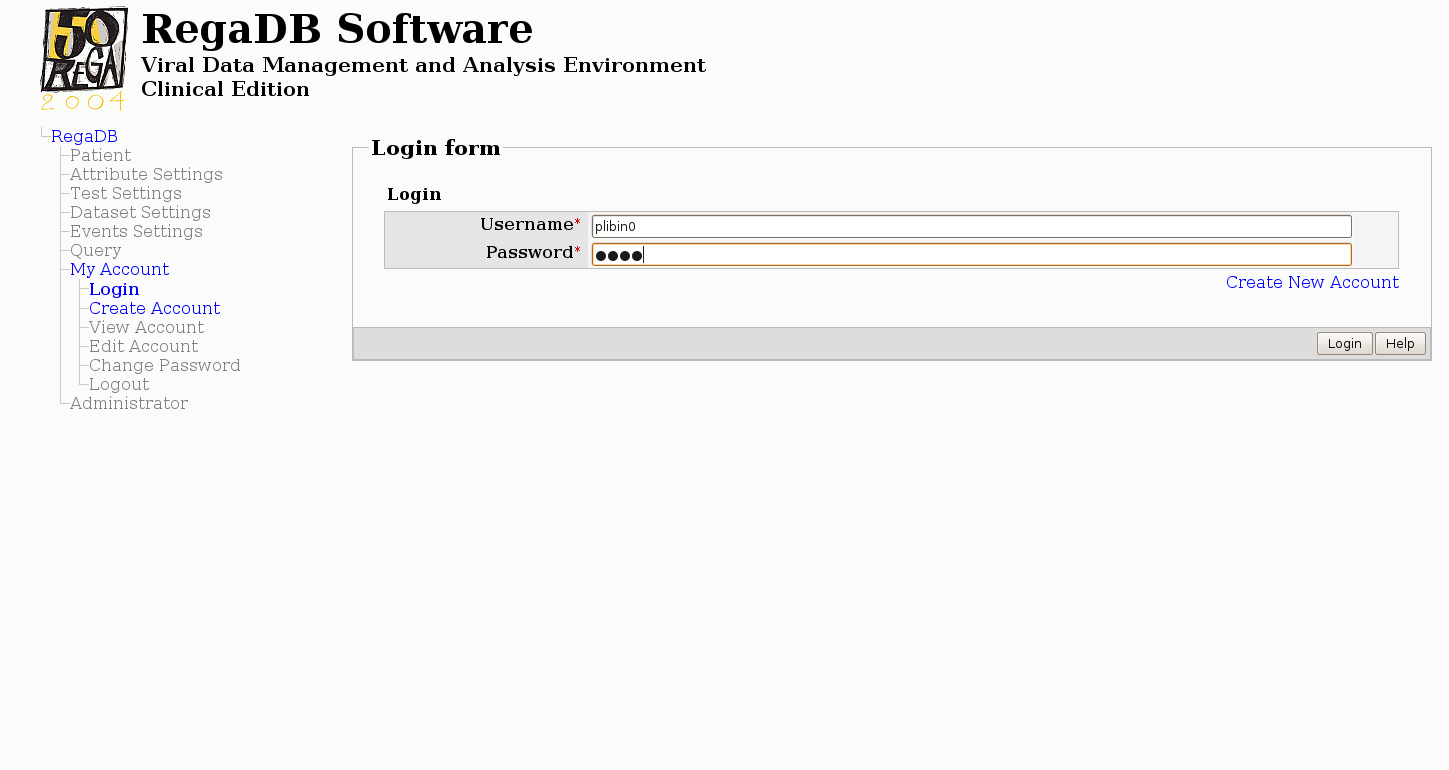
\includegraphics[width=15cm] {pics/auxilary/aux_1.png}}
\\
\vspace{0.5cm}~ \\ \centerline{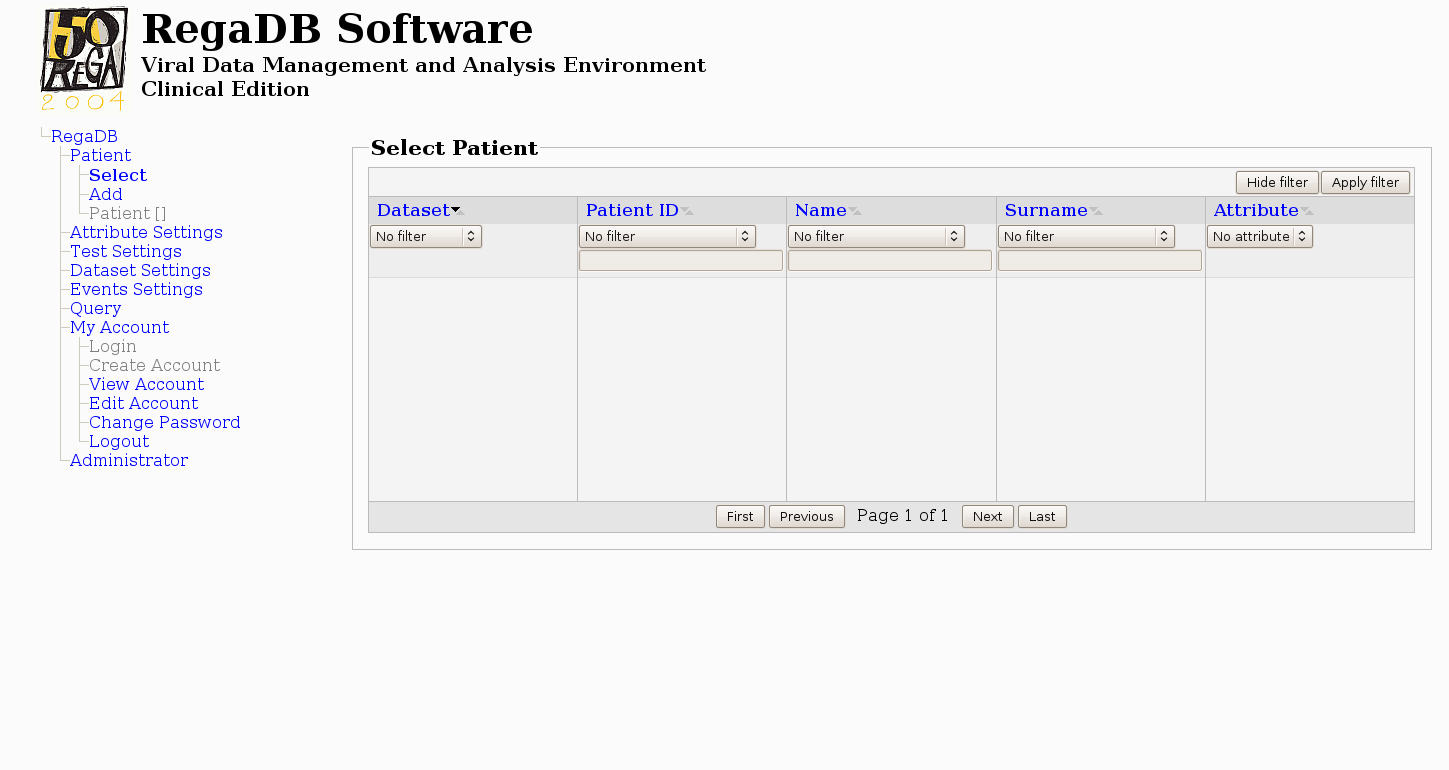
\includegraphics[width=15cm] {pics/auxilary/aux_2.png}}
\\
Navigate to the Administrator, Update from RegaDB Server page.
\\
\vspace{0.5cm}~ \\ \centerline{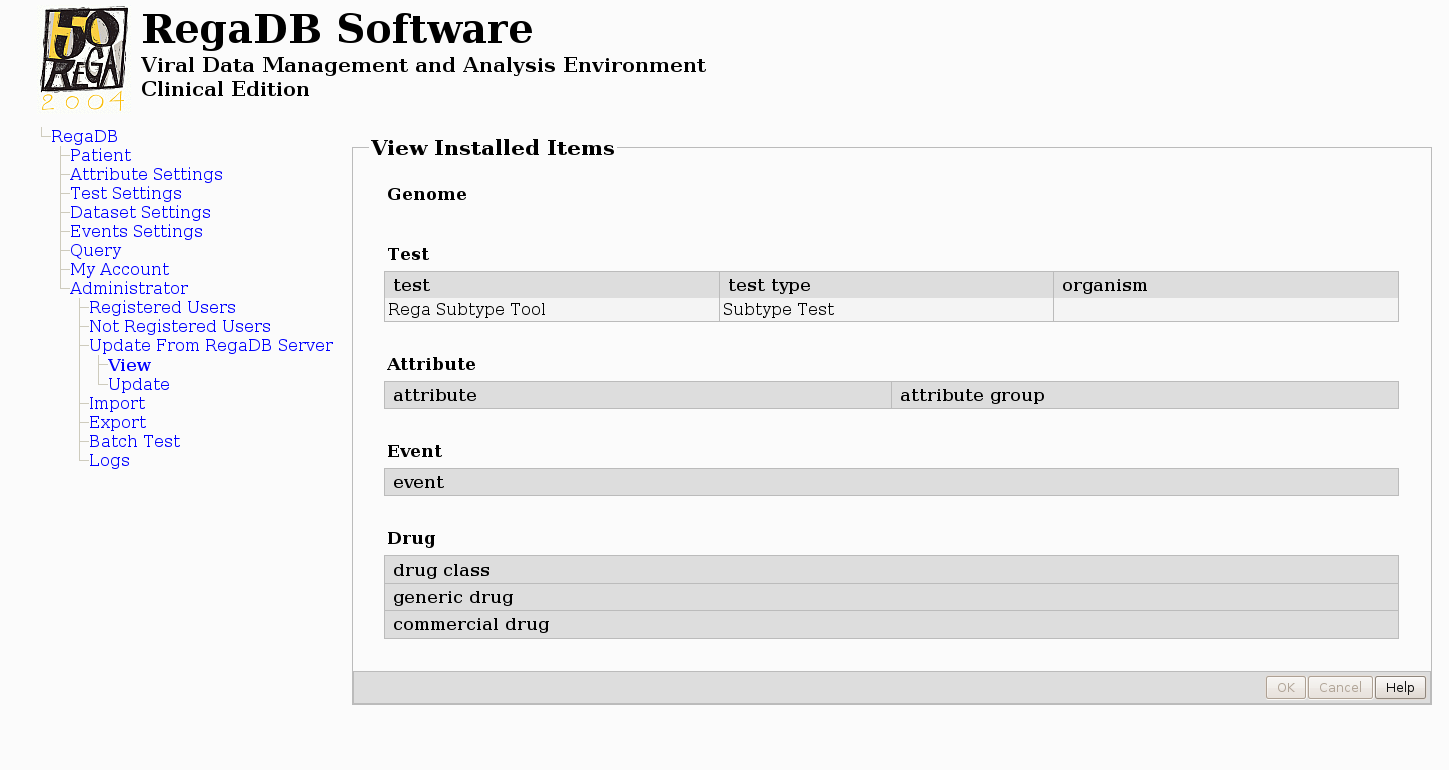
\includegraphics[width=15cm] {pics/auxilary/aux_3.png}}
\\
Click on Update, and a simulation update will be performed. This might take a few minutes, depending on your internet connection speed.
\\
\vspace{0.5cm}~ \\ \centerline{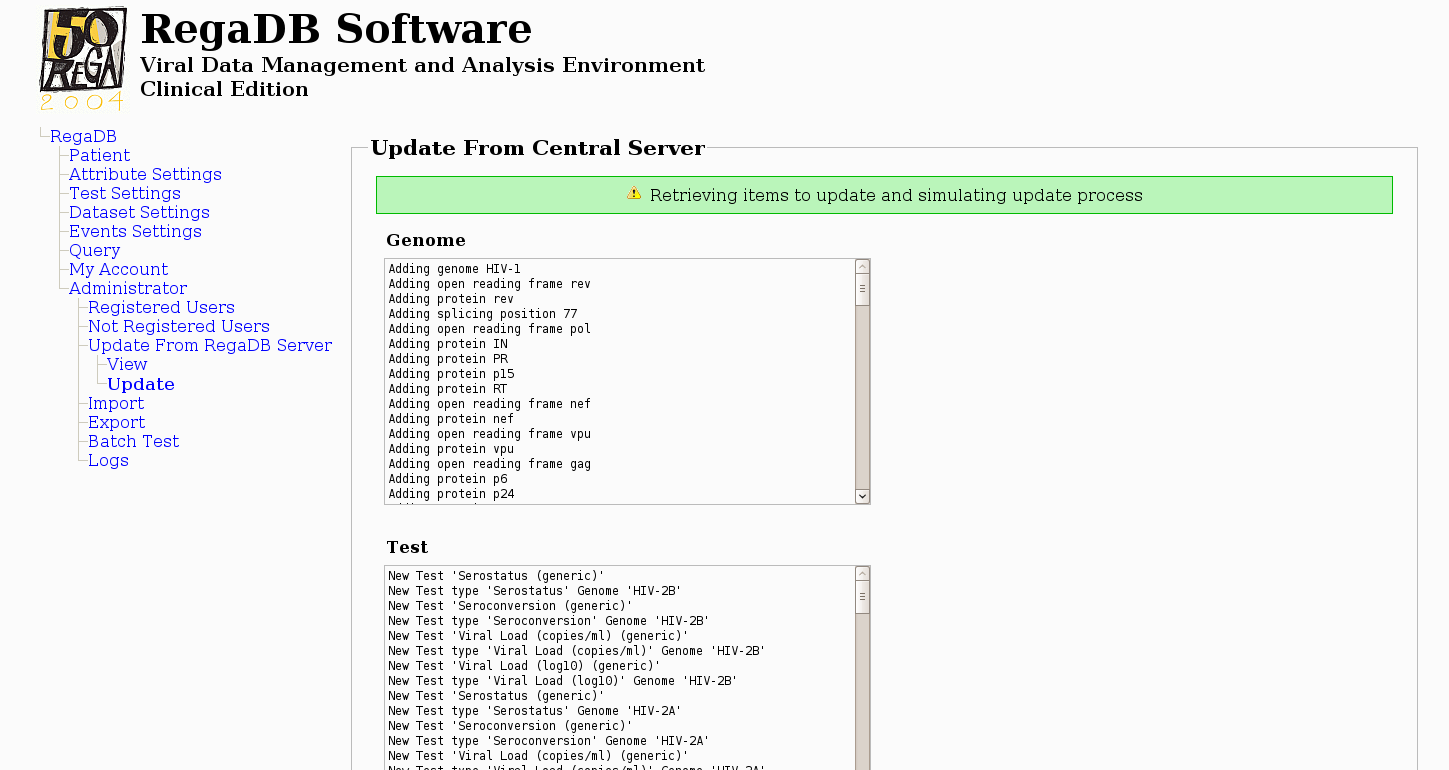
\includegraphics[width=15cm] {pics/auxilary/aux_4.png}}
\\
Click \textbf{OK} to confirm this simulation and to load the items into your local RegaDB instance. Again, this procedure might take a few minutes.
\\
\vspace{0.5cm}~ \\ \centerline{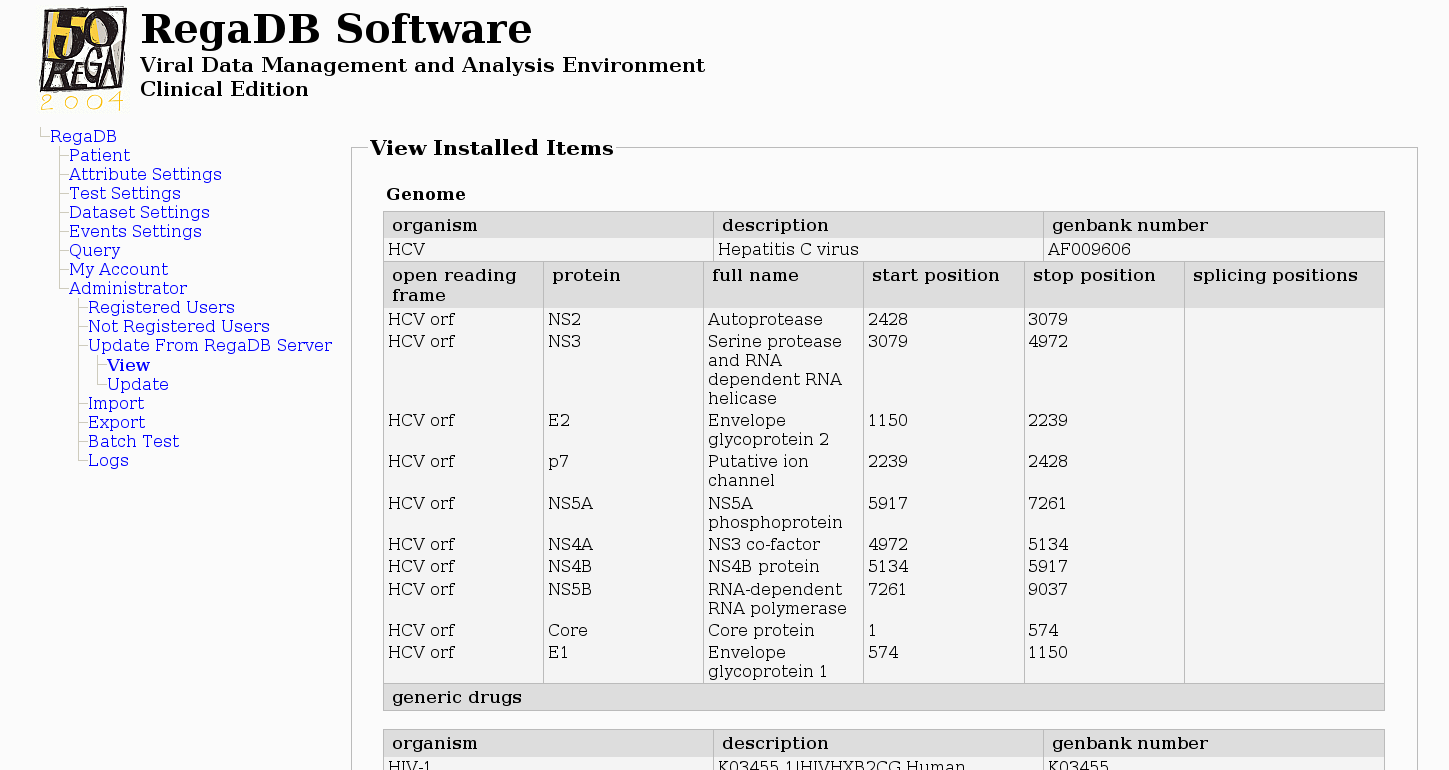
\includegraphics[width=15cm] {pics/auxilary/aux_5.png}}
\\
\section{Add a Dataset}
Navigate to the Administrator, Dataset settings menu, and add a new Dataset to the system.
\section{Contamination tool}
\subsection{Approximating distribution parameters}
The contamination tool uses both inter- and intra-patient sequence distance distributions. These distributions can be configured for multiple regions within a genome. Usually, using the precomputed values (such as offered on our website (TODO add link to our website)) is sufficient, however, it is also possible to esitimate these values on a existing database.
This is done by sampling a subset of all inter- and intra-patient sequence distances in the database, and afterwards fitting these distances on a log-normal distribution.

To sample the sequences distances for inter- or intra-patient run the SampleDistances program (located in regadb-analyses/src/net/sf/regadb/contamination/), this program accepts the following arguments:
\begin{itemize}
\item username 
\item password 
\item csv outputfile (eg.: outputfile.csv) 
\item outputType (intra-patient=I, inter-patient=O) 
\item ORF (eg.: pol) 
\item region range relative to the ORF (eg.: 169-1786) 
\end{itemize}

After sampling the distances, the approximation script can be used to fit the distances on a log-normal distribution. This script requires both an inter- and intra-patient distances csv file. The script can be found in regadb-analyses/src/net/sf/regadb/contamination and can be invoked with the following command and arguments:
\\
\textbf{Rscript regadb-analyses/src/net/sf/regadb/contamination/approximate\_distributions.R --intra intra.csv --inter inter.csv}
